\documentclass[a4paper, 12pt]{article}

\usepackage{graphicx}
\graphicspath{ {./} }


\newcommand{\templates}{./template}
\usepackage[a4paper, margin=2.5cm]{geometry}

\usepackage{enumitem}
\setlist[itemize]{noitemsep}
\setlist[enumerate]{noitemsep}

\let\oldpar\paragraph
\renewcommand{\paragraph}[1]{\oldpar{#1\\}\noindent}
\usepackage{graphicx}
\usepackage{hyperref}
\usepackage{makecell}

\newcommand{\settitolo}[1]{\newcommand{\titolo}{#1\\}}
\newcommand{\setmembri}[1]{\newcommand{\membri}{#1\\}}
\newcommand{\setanno}[1]{\newcommand{\anno}{#1\\}}
\newcommand{\setdescrizione}[1]{\newcommand{\descrizione}{#1\\}}

\newcommand{\makefrontpage}{
	\begin{titlepage}
		\begin{center}


		{\Large Relazione Progetto di Tecnologie Web}\\[6pt]

		\vspace{1.5cm}
		{\LARGE\titolo}

		\vfill

		\begin{tabular}{r | l}
		\multicolumn{2}{c}{\textit{Informazioni}}\\
		\hline

		\ifdefined\membri
			\textit{Membri del gruppo} &
			\makecell[l]{\membri}\\
		\else\fi

		\textit{Anno scolastico} & \anno

		\end{tabular}

		\vspace{2cm}

		\ifdefined\descrizione
		Descrizione
		\vspace{6pt}
		\hrule
		\descrizione
		\else\fi
		\end{center}
	\end{titlepage}
}

%package
\usepackage[table,xcdraw]{xcolor}


\settitolo{PNG Cinema}
\setmembri{Matteo Galvagni (1224451)\\Antonio Stan (1225426)\\Michele Gatto (1224458)\\Giovanni Cristellon (1216730)}
\setanno{2021-2022}
\setlink{http://tecweb.studenti.math.unipd.it/magalvag/}
\setutentebase{Username: user, Password: user}
\setutenteadmin{Username: admin, Password: admin}
\setdescrizione{Relazione PNG Cinema - Tecnologie Web}

\renewcommand*\contentsname{Indice}

\begin{document}

\makefrontpage
\tableofcontents
\clearpage

\section{Introduzione}
Il progetto in esame ha lo scopo di creare un sito web per il cinema fittizio "PNG Cinema" allo scopo di facilitare il processo di acquisto dei biglietti (saltando la fila nella biglietteria fisica) nonchè
il reperimento di informazioni utili per quanto concerne la programmazione di film nell'immediato futuro.
Altre informazioni che dovranno essere presenti nel sito riguardano il costo dei biglietti (ed eventuali sconti), dove contattare il cinema in caso di domande o problemi e come raggiungere fisicamente il cinema.
Trattandosi di un cinema locale e non facente parte di una catena, è prevista anche una parte del sito (accessibile ai soli utenti con i privilegi di amministratore) per l'inserimento manuale delle proiezioni in programma.

\section{Analisi dei Requisiti}
\subsection{Utenza target}
Si individuano due particolari tipologie di clienti target:
\begin{itemize}
    \item Utenti "frettolosi": sono clienti che, a poco tempo dall'inizio della proiezione di interesse e volendo saltare la fila alla biglietteria fisica, accedono al sito per acquistare rapidamente un biglietto.
    \\\item Utenti "ordinari": sono utenti interessati a reperire informazioni circa le proiezioni in programma nelle prossime settimane, il costo dei biglietti (ed eventuali convenzioni) e l'ubicazione del cinema.
\end{itemize}
I clienti target, in ogni caso, hanno un'età media nel range dei 25-30 anni. La categoria di clienti oltre i 65 anni, che gode di particolari sconti, preferisce in modo quasi assoluto l'acquisto in biglietteria fisica.
Esistono inoltre gli utenti "amministratori" del cinema, che vogliono la possibilità di inserire film e proiezioni all'interno del sito.
\subsection{Search Engine Optimization}
Per ogni pagina sono state scelte delle keyword coerenti, che fossero presenti nella relativa pagina.\\
In ogni pagina il nome del cinema è riportato nel tag \textit{h1}, essendo la ricerca per nome del cinema una delle più probabili.\\
Keyword e tag di intestazione sono in ogni caso stati scelti in base alle parole che possano con maggiore probabilità apparire in una ricerca da parte dei clienti.
Inoltre, tutto il codice HTML e CSS è stato validato.
Non viene utilizzato Javascript per riempire di contenuti il sito, ma solo per alcune funzionalità di comodità dedicate agli utenti.

\clearpage

\subsection{Ricerche probabili}
Per massimizzare la visibilità in un motore di ricerca, il sito deve rispondere a delle query eseguite da utenti che già conoscono il nostro cinema.
Fondamentale è che risponda agli utenti interessati alla visione degli ultimi film usciti a Padova. Infine deve soddisfare le richieste di coloro che cercano una funzionalità di acquisto rapido di biglietti per i film.\\
Di seguito vengono riportate le più probabili tra le ricerche possibili a cui dovrebbe rispondere il sito:

\begin{itemize}
\item cinema padova;
\item pngcinema;
\item pngcinema padova;
\item acquisto biglietto film;
\item acquisto rapido biglietto film;
\item ultime uscite film.
\end{itemize}

\newpage

\section{Progettazione}
Il sito web è stato progettato fin da subito per rispondere alle tre domande "Dove mi trovo?", "Dove posso andare?" e "Cosa c'è in questa pagina?": è stato utilizzato un layout "classico", con menù in testa ad ogni pagina e con subito sotto le breadcrumbs che indicano all'utente dove si trova e che percorso ha effettuato per arrivarci. Oltre un certo punto di rottura, il menù collassa ad un menù ad hamburger per meglio adattarsi ai dispositivi con schermi di piccola dimensione.\\
\\In fondo ad ogni pagina è presente un footer che riassume gli orari di apertura del cinema e che linka alla pagina dei contatti, in caso un utente abbia scrollato fino in fondo e abbia la necessità di visualizzare la pagina dei contatti (non obbligandolo a ri-scrollare fino al menù).

\subsection{Mappa sito}
\begin{center}
    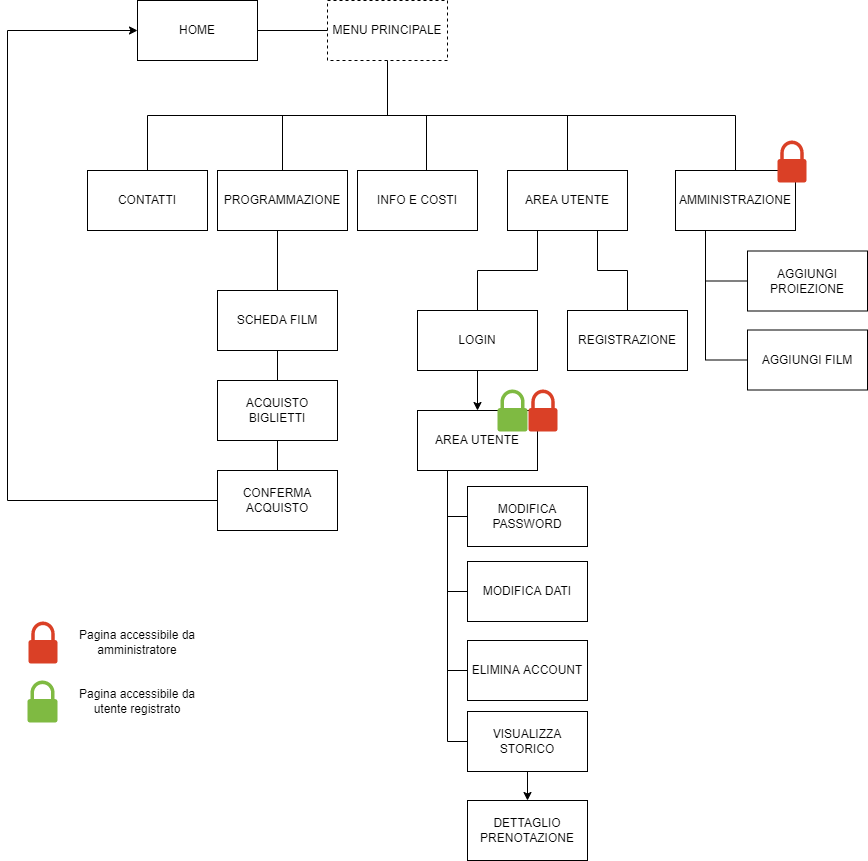
\includegraphics[scale=0.5]{mappasito}
\end{center}

\subsection{Organizzazione pagine}
Le pagine del sito sono organizzate per "argomento", raggruppando le informazioni più interessanti per i clienti.
Le pagine raggiungibili dal menù sono:
\begin{itemize}
    \item Home
    \item Contatti
    \item Programmazione
    \item Info e Costi
    \item Area Utente
    \item Amministrazione
\end{itemize}
Altre pagine raggiungibili dalla pagina "Programmazione" sono "Scheda Film" e successivamente "Conferma Acquisto" all'acquisto di uno o più biglietti.

\subsection{Acquisto rapido}
La pagina Home contiene, fra le altre cose, un form che consente l'acquisto rapido (cioè senza passare per programmazione/scheda film/prenotazione) di biglietti per una particolare proiezione. Questa sezione è presente nella zona "above the fold", perchè pensata in particolar modo per la categoria di utenti "frettolosi" che nella stragrande maggioranza dei casi acquisterà i biglietti da dispositivo mobile (essendo probabilmente già fuori casa). In ogni caso, la possibilità di acquistare rapidamente dei biglietti direttamente dalla pagina Home risulta particolarmente comoda anche per clienti abituali o che comunque sanno già cosa vogliono.
\subsection{Selezione posti}
All'interno del sito sono presenti due modalità per acquistare i biglietti: la prima prevede la selezione grafica dei posti scelti all'interno di una sezione apposita; la seconda, più accessibile, prevede la semplice selezione dei posti come coppia fila-numero posto. In entrambe le modalità è richiesto all'utente di specificare quanti biglietti (e di che tipo) voglia acquistare.

\newpage
\subsection{Database}
Di seguito lo schema concettuale del database:

\begin{center}
    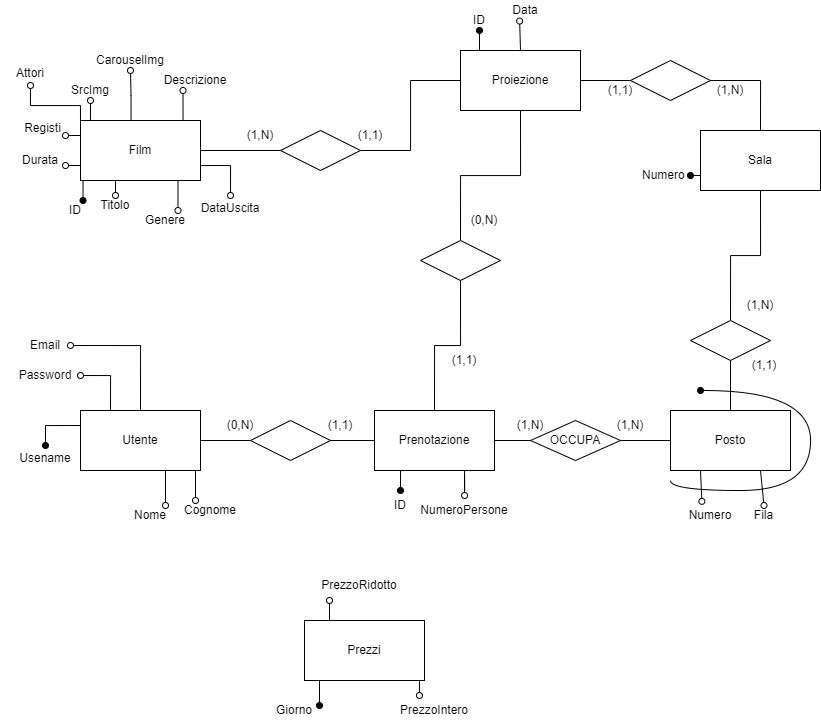
\includegraphics[scale=0.5]{database}
\end{center}

In particolare, valutato il fatto che in una situazione reale, raramente vengono cambiati i layout di sale e le numerazioni dei posti, si è deciso che queste rimarranno fisse e non modificabili. Inoltre sono state applicate alcune semplificazioni in sede di progetto:
\begin{itemize}
\item ogni sala ha la stessa quantità, numerazione e layout di posti;
\item i prezzi non sono modificabili dagli amministratori (se non direttamente da un strumento come phpMyAdmin).
\end{itemize}


\section{Implementazione}
È stato scelto di sviluppare il sito utilizzando HTML5, non avendo particolari esigenze di compatibilità vista l'utenza molto giovane.
Avendo prestato particolare attenzione alla categoria di utenti "frettolosi", e dunque all'accesso del sito da mobile, fin da subito ogni unità di misura utilizzata in CSS è stata relativa per permettere la corretta responsività del sito (fatta eccezione per la massima larghezza del body, 1024px, e i bordi di alcuni elementi grafici).
Sono stati implementati diversi controlli sia lato client (Javascript) sia lato server (PHP) ad ogni input dell'utente.
Ogni input inoltre è sottoposto a controllo, lato server, dell'assenza di codice malevolo per evitare JS/SQL injections.
La connessione al database è stata effettuata implementando il design pattern Singleton.\\\\
In alcune parti del sito abbiamo ritenuto opportuno l'utilizzo di AJAX: nella pagina Home ci consente di riempire dinamicamente i campi di selezione della sezione di acquisto rapido; nella pagina di amministrazione consente di visualizzare in modo dinamico e senza ricaricare la pagina la lista di film e proiezioni.
Nella pagina di amministrazione, inoltre, per inserire un film o una proiezione all'interno del sito si apriranno dei popup: questa scelta è stata fatta per rendere l'esperienza utente dell'amministratore simile a quella di una webapp, contrapposta all'alternativa di aprire una nuova scheda o modificare la pagina ad ogni richiesta di inserimento, giudicate soluzioni piuttosto invasive; in ogni caso questa pagina è stata dotata di link nascosti per rendere la navigazione piacevole anche da screenreader. La visualizzazione delle tabelle di questa pagina, da mobile, è stata mantenuta con uno scorrimento orizzontale delle singole tabelle: questo, seppure non ottimale, è stato considerato migliore all'adattamento verticale di tabelle con molti film e proiezioni che ne diminuivano di molto la leggibilità e aumentavano esponenzialmente la lunghezza dello scroll necessario per arrivare a fondo pagina; è stata inoltre pensata come soluzione accettabile per via della prevalenza di utilizzo di questa pagina da desktop.\\\\
La pagina di amministrazione consente l'inserimento nel database di film e proiezioni; per inserire un film è richiesto l'inserimento di due immagini di locandina (una orizzontale per il carosello presente in Home e una in verticale per la visualizzazione nelle cards): per semplicità di implementazione tale inserimento è di tipo testuale, e richiede infatti il nome del file (con estensione, es. "sonic2-vertical.jpg") dell'immagine desiderata che deve essere caricata manualmente nella cartella /images.
\\\\Il sito è stato testato su tutti i browser maggiormente utilizzati (Chrome, Firefox, Opera, Safari, Brave, Edge). È stato ritenuto ragionevole, tuttavia, omettere la compatibilità del sito con il browser Internet Explorer sia per l'utenza target molto giovane sia perchè il browser in questione è stato abbandonato dall'azienda di produzione in favore di Edge (meno dello 0.5\% degli utenti utilizza IE in Italia ad aprile \\di quest'anno, fonte https://gs.statcounter.com/browser-market-share/all/italy).
\newpage
\section{Accessibilità}
Il codice HTML5 è stato validato utilizzando il servizio di W3C https://validator.w3.org/.
Il codice CSS è stato validato utilizzando il servizio di W3C https://jigsaw.w3.org/css-validator/.
Sono stati controllati i contrasti di ogni colore utilizzando il servizio \\https://webaim.org/resources/contrastchecker/.
Sono stati interiti tag opportuni circa la modellazione del contenuto del sito e non per fini estetici; sono state inseriti abbreviazioni, testi nascosti, descrizioni di immagini e tag aria dove necessario.
Sono stati generati report con LightHouse di Chrome che non hanno evidenziato particolari criticità, se non per la grandezza delle immagini che comunque, essendo locandine, si è ritenuto ragionevole non
diminuirne la risoluzione.
\begin{center}
    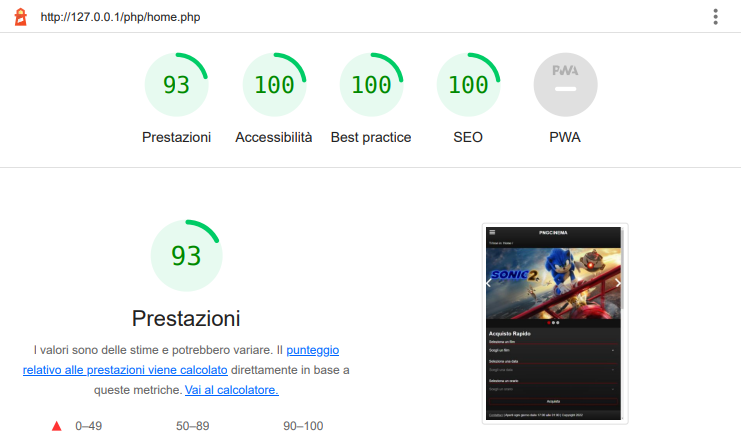
\includegraphics[scale=0.4]{home}
\end{center}
È stato controllato come le pagine reagiscono rispetto a diversi disturbi visivi; di seguito alcuni esempi.
\begin{center}
    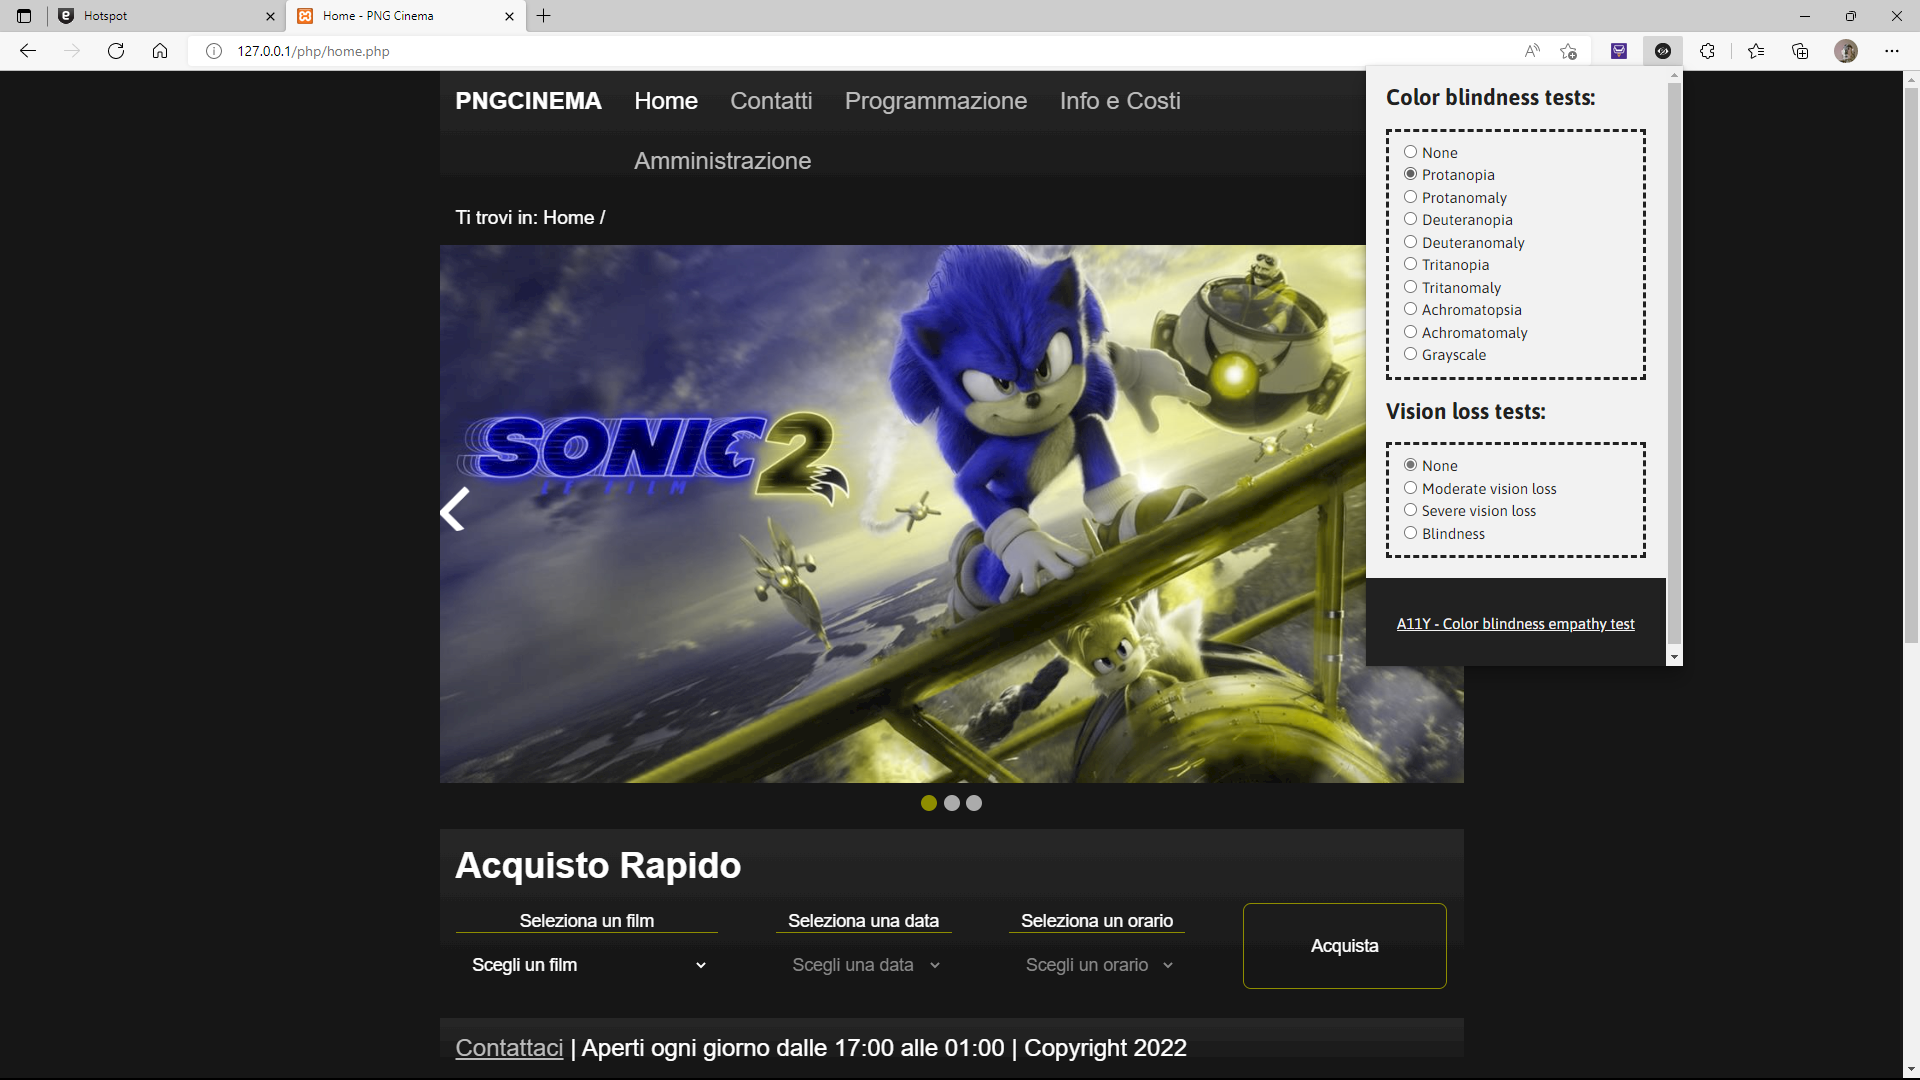
\includegraphics[scale=0.1]{protanopia}
    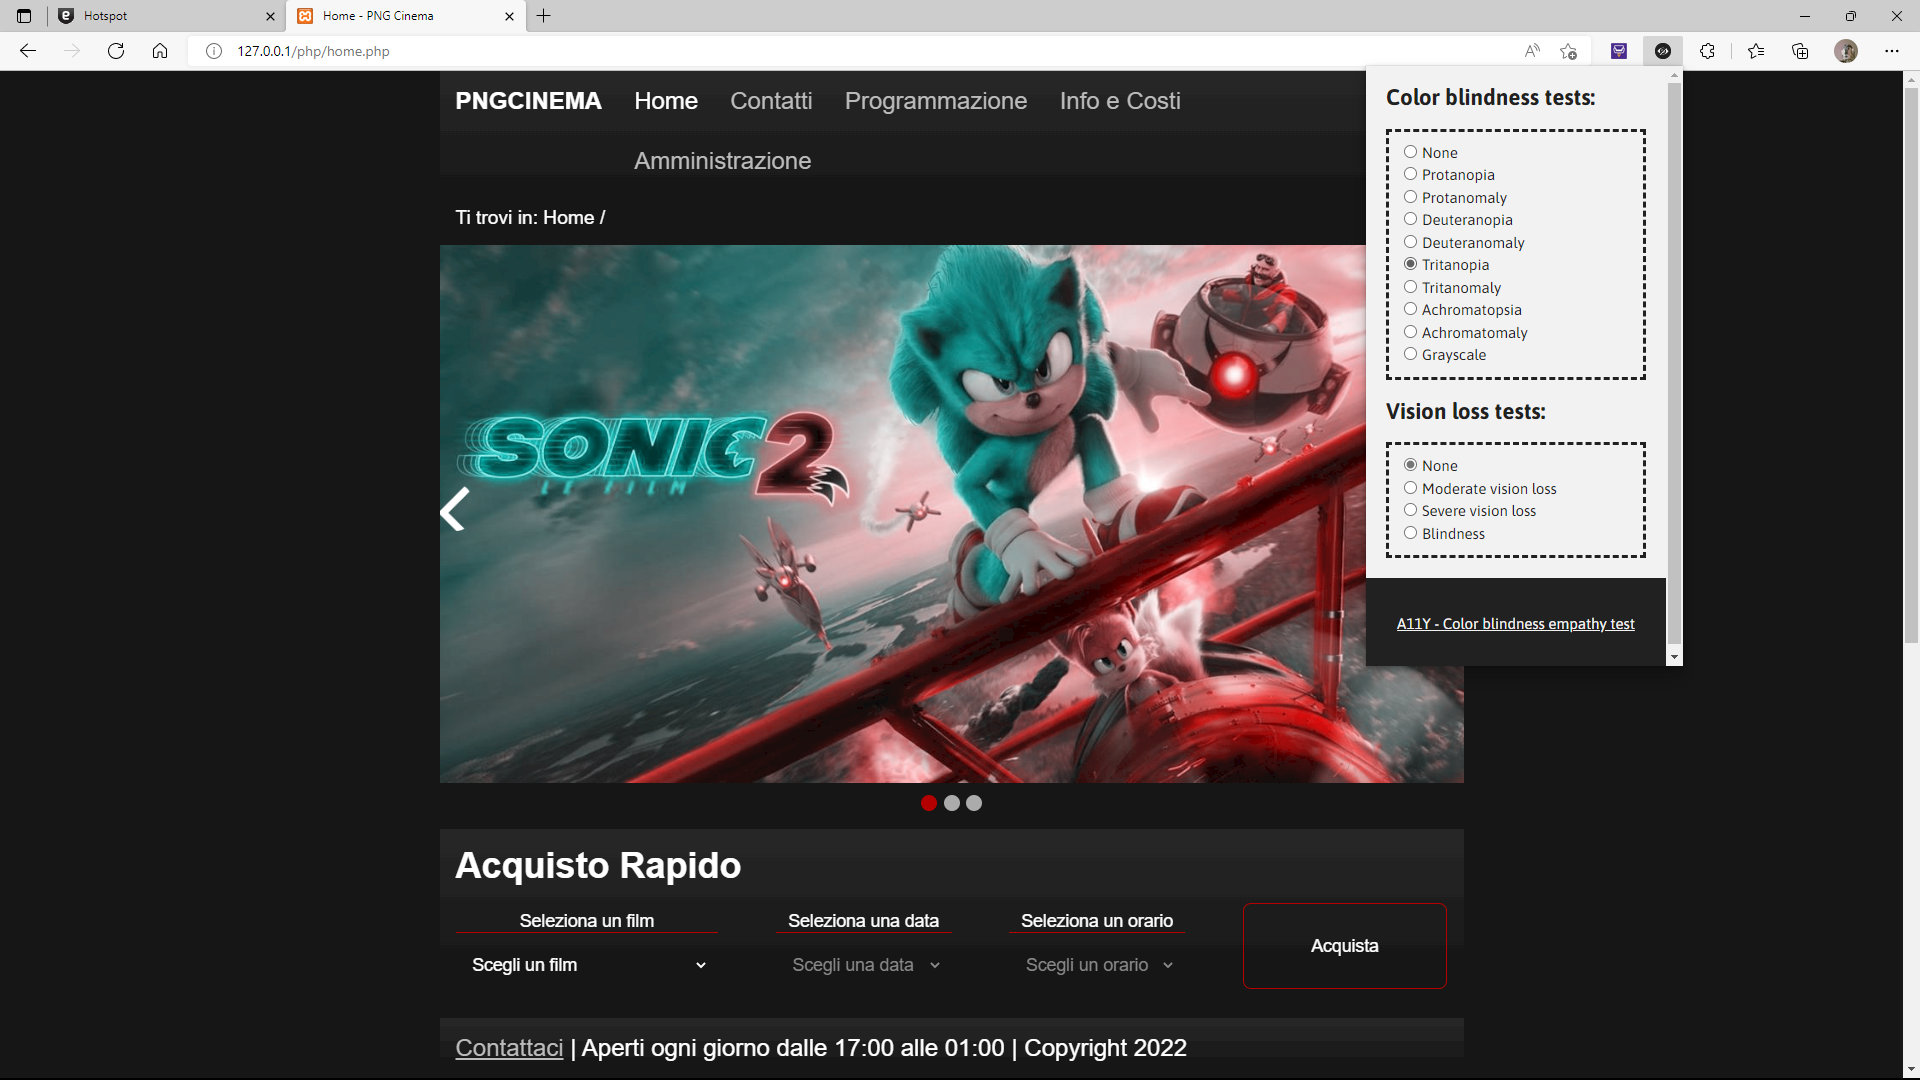
\includegraphics[scale=0.1]{tritanopia}
\end{center}

Il sito è stato testato nella sua interezza sia con screenreader di default di Windows sia con estensione per browser.
In ogni pagina del sito sono presenti dei link nascosti che consentono agli utenti che navigano spostandosi tra link di saltare al contenuto interessante della pagina evitando elementi grafici o inutili.
Il carosello presente in home è stato reso scorribile sia con bottoni cliccabili, sia con frecce della tastiera, sia con link a fondo carosello.
\\\\
Vista la quantità non indifferente di attori, registi e in generale parole inglesi sia nel titolo che nella descrizione dei film, è stato pensato di consentire all'amministratore l'inserimento di tali parole delimitato da caratteri di "escape" in modo che vengano filtrati dal codice PHP sostituendoli con appositi tag che specifichino la lingua di quel pezzo di testo (in questo caso è stato scelto di indicare le parole inglesi tra parentesi grafe, es. "\{Spiderman\}").
\section{Note}
\subsection{Validazione email}
In fase di registrazione agli utenti è richiesto di inserire una email. Consci del fatto che l'unico modo sicuro al 100\% per validare un indirizzo email è tramite l'invio di una mail a tale indirizzo con un codice di controllo è stato deciso di limitare i controlli di questo input al solo check della presenza del carattere chiocciola, dato che utilizzare una qualsiasi espressione regolare per effettuare la validazione sarebbe risultato probabilmente sbagliato. L'invio del codice tramite email è stato omesso per eccessiva complessità d'implementazione a fronte di un guadagno minimo e mancanza di tempo, ma è sicuramente un'aggiunta che andrebbe fatta in un sito reale.
\subsection{Pagine statiche}
Pur esistendo una pagina puramente statica all'interno del sito (pagina contatti) è stato ritenuto accettabile fornire tale pagina tramite del codice PHP, perchè a fronte di un guadagno veramente minimo in termini di velocità di caricamento si sarebbe persa la divisione del codice tra template HTML base delle pagine e contenuto inserito in maniera dinamica in solamente quella pagina.
Facendo così è possibile modificare la template del sito (per esempio, se fosse necessario cambiare il footer) tramite un solo file, con la sicurezza che la modifica sia applicata in ogni pagina. Facendo diversamente le modifiche degli elementi presenti in ogni pagina sarebbero dovute essere scritte due volte, senza garanzia di coerenza tra di loro.
\subsection{CSS non minimizzato}
È stato ritenuto opportuno per lo scopo di questo progetto non minimizzare il codice CSS per favorirne la leggibilità.
\subsection{Installazione}
Per l'installazione su altro server è necessario modificare il file SingletonDB.php presente in /php/utils inserendo i dati di accesso al proprio database (HOST, USERNAME, PASSWORD e NAMEDB).



\newpage
\section{Divisione del lavoro}
\subsection{Matteo Galvagni}
\begin{itemize}
    \item Template (HTML + CSS)
    \item Home (HTML + CSS + PHP + JS)
    \item Programmazione (PHP Parziale)
    \item Area Utenti - Registrazione (PHP Parziale)
    \item Controlli Input Area Utenti (JS + PHP)
    \item Pagine di errore (HTML + CSS + PHP)
    \item Relazione
\end{itemize}
\subsection{Antonio Stan}
\begin{itemize}
    \item Area utenti - Login (HTML + CSS + PHP)
    \item Area utenti - Registrazione (HTML + CSS + PHP)
    \item Area utenti - Modifica (HTML + CSS + PHP)
    \item Programmazione (PHP Parziale)
    \item Database (Parziale)
\end{itemize}
\subsection{Michele Gatto}
\begin{itemize}
    \item Scheda Film (HTML + CSS + PHP)
    \item Prenotazione (HTML + CSS + PHP + JS)
    \item Programmazione (PHP)
    \item Database
    \item Info e Costi (HTML + CSS + PHP)
    \item Home (PHP Parziale)
    \item Validazione
\end{itemize}
\subsection{Giovanni Cristellon}
\begin{itemize}
    \item Area amministrazione (HTML + CSS + PHP + JS)
    \item Contatti (HTML + CSS + PHP)
    \item Info e Costi (HTML Parziale)
    \item Revisione Accessibilità
\end{itemize}

\section{Conclusioni}
In questo progetto è stata prestata maggiore attenzione alla struttura del sito rispetto che al funzionamento nel complesso: per questo motivo, parti come il pagamento di un biglietto non sono state implementate
per mancanza di tempo e perchè non di diretto interesse. Possibili aspetti migliorativi potrebbero riguardare l'upload di immagini direttamente dalla pagina amministrazione (attualmente manuale) e l'invio di e-mail con codici per la verifica dell'indirizzo e-mail in fase di registrazione.\\
Le maggiori criticità riscontrate durante lo sviluppo del progetto sono di carattere organizzativo, quali l'iniziale assenza di revisioni del codice prima di effettuarne il merge e l'assenza di scadenze precise prima della quale consegnare le proprie parti.
\end{document}
